\documentclass[letterpaper,10pt]{article}
\usepackage[utf8x]{inputenc}
\usepackage{amsmath,amsfonts,amsthm,amssymb}
\usepackage{mathrsfs} %script font
\usepackage{graphicx}
\usepackage{multirow}
\usepackage{fancyhdr}
\usepackage{extarrows}
\usepackage[margin=1in]{geometry}
\usepackage{framed}
\usepackage{tikz}

\usepackage[english]{babel}
\usetikzlibrary{arrows}


\def \B {\mathscr{B}}
\def \F {\mathscr{F}}
\def \Q {\mathbb{Q}}
\def \R {\mathbb{R}}
\def \E {\mathbb{E}}
\def \M {\mathbb{M}}
\def \N {\mathbb{N}}

\newcommand{\Ac}{{\cal A}}
\newcommand{\Bc}{{\cal B}}
\newcommand{\Cc}{{\cal C}}
\newcommand{\Ec}{{\cal E}}
\newcommand{\Fc}{{\cal F}}
\newcommand{\Gc}{{\cal G}}
\newcommand{\Lc}{{\cal L}}
\newcommand{\Mc}{{\cal M}}
\newcommand{\Nc}{{\cal N}}
\newcommand{\Rc}{{\cal R}}
\newcommand{\Pc}{{\cal P}}
\newcommand{\Tc}{{\cal T}}

\tikzset{
  treenode/.style = {align=center, inner sep=0pt, text centered,
    font=\sffamily},
  arn_n/.style = {treenode, circle, white, font=\sffamily\bfseries, draw=black,
    fill=black, text width=1.5em},% arbre rouge noir, noeud noir
  arn_r/.style = {treenode, circle, red, draw=red,
    text width=1.5em, very thick},% arbre rouge noir, noeud rouge
  arn_x/.style = {treenode, rectangle, draw=black,
    minimum width=0.5em, minimum height=0.5em}% arbre rouge noir, nil
}


\begin{document}
\pagestyle{fancy}
\lhead{}
\chead{}
\rhead{}
\author{Tianyi Chen^{*}, Guanyi Wang, Bowen Li, Mingyue Gao}
\title{CS 676 Machine Learning Homework 1-1a}
\maketitle
\nocite{*}



\section{Bayesian Linear Regression}
You work at a prestigious investment bank, and your job as an analyst is to build a model to predict the price of company $Y$'s stock given the current prices for companies $A,B,C$ and $D$. You will be receiving new price data every millisecond. You would like to build a model that continuously updates its beliefs about $\omega$ as you receive new data. You think that a Gaussian distribution approximately captures your beliefs a priori about the parameter $\omega$. Suppose the prior distribution is parameterized with the mean vector $\mu_0$ and covariance matrix $\Sigma_{0}$. The likelihood model is the standard linear regression likelihood:
\begin{equation}\label{}
 Y_i \sim X_i^T \omega + \Nc (0, \sigma^2)
\end{equation}

\begin{framed}
\textbf{a. 10 points:} After n observations, what will be our prior distribution over w at time $n+1$ (what is the distribution and what are its parameters)?
\end{framed}
By formula (1), let us define noise as $\epsilon \sim \Nc (0, \sigma^2)$, then we have
$$
Y_i = X_i^T \omega + \epsilon.
$$
From the conditions above, we suppose that the prior distribution of parameter $\omega$ satisfies: $\omega \sim \Nc (\mu_0, \Sigma_0)$, let us define $\omega_{1} = \omega; \mu_1 =\mu_0; \Sigma_1 = \Sigma_0$ as the prior of the 1st step, that is to say: $P(\omega_{1}) = \Nc (\omega_1 | \mu_1, \Sigma_1)$. Now let us focus on the 1st step: our goal is to compute the prior of the second step ( that is to say, the posterior of $\omega_1$ after one observation ), since we have $P(Y_1|X_1,\omega_1,\sigma^2 ) = \Nc (Y_1|X_1^T \omega_1, \sigma^2)$, then by:
$$
P(\omega_1 | X_1, Y_1, \sigma^2) \propto P(\omega_1 | \sigma^2) P(Y_1| X_1, \omega_1, \sigma^2)
$$
$$
= \Nc (\omega_1 | \mu_1, \Sigma_1) \Nc (Y_1|X_1^T \omega_1, \sigma^2) = \Nc(\omega_1| \mu_{1}, \Sigma_{1})
$$
in which
\begin{align*}
& \Sigma_{1} = \sigma^2(\sigma^2 \Sigma_0^{-1} + X_1^TX_1)^{-1}\\
& \Sigma_{1}^{-1} = \Sigma_0^{-1} + \frac{1}{\sigma^2} X_1^TX_1 \\
& \mu_{1} = \Sigma_{1} \Sigma_0^{-1} \mu_0 + \frac{1}{\sigma^2} \Sigma_{1} X_1^T Y_1 \\
\end{align*}
Then let $\omega_2 = \omega_1 | X_1, Y_1, \sigma^2$ with the prior of $\mu_2$ is $\mu_{1}$ and prior of $\Sigma_2$ is $\Sigma_{1}$, therefore, we have:
$$
\omega_2 \sim \Nc (\mu_2, \Sigma_2), \text{ and } P(\omega_2) = \Nc (\omega_2| \mu_2, \Sigma_2).
$$
Repeat the ways above, we could get the prior of $i+1$th step under the $i$th step. Now, for the $n+1$th step, the prior of the $n+1$th step is the posterior of $n$th step, if we have the posterior of $n$th step as $\omega_n \sim \Nc(\mu_n, \Sigma_n)$, then by the ways above, we get $\omega_{n+1}\sim \Nc(\mu_{n+1}, \Sigma_{n+1})$ in which
\begin{align*}
& \Sigma_{n+1}  = \sigma^2(\sigma^2 \Sigma_n^{-1} + X_n^TX_n)^{-1}\\
& \Sigma_{n+1}^{-1} = \Sigma_n^{-1} + \frac{1}{\sigma^2} X_n^TX_n \\
& \mu_{n+1} = \Sigma_{n+1} \Sigma_n^{-1} \mu_n + \frac{1}{\sigma^2} \Sigma_{n+1} X_n^T Y_n \\
\end{align*}

\begin{framed}
\textbf{b. 5 points:} Given $X_{n+1}$ and the prior density you computed above, write down the full posterior predictive distribution over $Y_{n+1}$.
\end{framed}
By formula (7.60) in Murphy's book, the posterior predictive distribution over $Y_{n+1}$ could be shown as:
$$
P(Y_{n+1}|X_{n+1}, \omega_{n+1}, \sigma^2) = \int \Nc (Y_{n+1}| X_{n+1}^T \omega_{n+1}, \sigma^2) \Nc(\omega_{n+1}| \mu_{n+1}, \Sigma_{n+1}) d\omega_{n+1}
$$

$$
= \Nc (Y_{n+1}| \omega_{n+1}^T X_{n+1}, \sigma_{n+1}^2 (X_{n+1}))
$$
where
$$
\sigma_{n+1}^2 (X_{n+1})) = \sigma^2 + X_{n+1}^T \Sigma_{n+1, N} X_{n+1}
$$

\begin{framed}
\textbf{c. 5 points:} Suppose we are unsure about our choice of hyperparameters $\mu_0$ and $\sigma_0$. To account for our uncertainty, we can use hierarchical Bayes and place some prior $\pi (\mu_0, \Sigma_0)$ over the hyperparameters. What estimation technique could we use to approximate the prior in the full hierarchical Bayes model?
\end{framed}

To account for our uncertainty of hyperparameter, for the first step, and the posterior of the first step could be
$$
P(\pi, \omega_1 | X_1, Y_1, \omega_1) \propto P(Y_1 | X_1, \omega_1, \sigma) P(\omega_1 | \mu_1,\Sigma_1) \pi(\mu_0, \Sigma_0).
$$
Then for each step( say step $i$ ), we \textbf{do not} directed define the prior of $i$th step $\omega_i$ as the posterior of $i-1$th step (say $( \omega_{i-1}| X_{i-1}, Y_{i-1}, \sigma )$); Instead, we define the prior of $i$th step as this:\\
(i) We have distribution of the posterior of $i-1$th step as
$$
( \omega_{i-1}| X_{i-1}, Y_{i-1}, \sigma ) = \omega_{i-1, \text{posterior}} \sim \Nc( \mu_{i-1, \text{posterior}}, \Sigma_{i-1, \text{posterior}})
$$
(ii) Then define the distribution of $i$th step as
$$
\omega_i \sim \Nc(\mu_i, \Sigma_i)
$$
in which $\mu_i, \Sigma_i$ are random variables, which satisfies:
$$
( \mu_i, \Sigma_i ) \sim \pi (\mu_{i-1, \text{posterior}}, \Sigma_{i-1, \text{posterior}})
$$
Therefore, we have the probability of $i$th prior $P(\omega_i)$ could be computed as
$$
P(\omega_i) = \int P(\omega_i | \mu_i, \Sigma_i) \pi (\mu_i, \Sigma_i | \mu_{i-1, \text{posterior}}, \Sigma_{i-1, \text{posterior}}) d\mu_i d\Sigma_i
$$
Then the posterior of $i$th step $\omega_i | X_i, Y_i, \sigma$ is
$$
P(\pi,\omega_i | X_i, Y_i, \sigma) \propto P(Y_i | X_i, \omega_i, \sigma) P(\omega_i)
$$
$$
\propto P(Y_i | X_i, \omega_i, \sigma) P(\omega_i | \mu_i, \Sigma_i) \pi (\mu_i, \Sigma_i | \mu_{i-1, \text{posterior}}, \Sigma_{i-1, \text{posterior}})
$$
In approximating the prior in the full hierarchical Bayes model, by Empirical Bayes or evidence approximate, we could find the hyperparameters maximizes the marginal likelihood as
$$
\hat{\pi} = \arg \max \{ \int P(Y | X, \omega, \sigma) P(\omega | \pi) d\omega  \}
$$

\begin{framed}
\textbf{d. 5 points:} You need to be able to predict $Y_{n+1}$ quickly, why is the full posterior predictive distribution a bad choice in this scenario? How could you approximate it? Under what condition is this approximation reasonable?
\end{framed}

Since full posterior predictive distribution requires to marginalize all the parameters, which is hard to compute. Since by part(c) above, we could compute $\hat{\pi}$ as an approximation, then we have $\hat{\pi} = \hat{\pi}(\hat{\mu_0},\hat{\Sigma_0} )$, then for the posterior of $\omega$ we have
$$
P(\omega | Y ) = P(Y| \omega ) P(\omega| \hat{\mu_0},\hat{\Sigma_0})
$$
And the condition of this approximation reasonable is that if the posterior is sharply peaked around our $\hat{\pi}$.

\begin{framed}
\textbf{e. 10 points:} After observing $10,000$ examples, your boss comes to let you know that the PhDs in the back have suggested that there may be a correlation between the influences that the stock prices for companies $A$ and $B$ or for companies $C$ and $D$ have on $Y$'s price, but they're not sure which. In fact, they're not even entirely sure that the correlation exists.\\
Let $\Mc_0$ denote the model in which there are no correlations between any of the weights in the model, $\Mc_{AB}$ denote the model in which the weights for $A$ and $B$ are correlated, and $\Mc_{CD}$ denote the model in which the weights for $C$ and $D$ are correlated. Assuming that all variances are $\sigma_0^2$ and all covariances are $\gamma_0^2$, how would you encode the beliefs of these three models in three different prior distributions?
\end{framed}

These three models can show the correlation between the free weight parameter in $\omega$. $\Mc_0$ means the four parameters are independent on each other.  $\Mc_{AB}$ means A,B has somewhat correlation, and  $\Mc_{CD}$ means C,D has somewhat correlation.
Therefore, there exist three forms of initial $\Sigma_0$:
$$
\Sigma_{0, AB} =
\left(
  \begin{array}{cccc}
    \sigma_0^2 & \gamma_0^2 & 0 & 0 \\
     \gamma_0^2 & \sigma_0^2 & 0 & 0\\
     0 & 0 & \sigma_0^2 & 0 \\
     0 & 0 & 0 & \sigma_0^2 \\
  \end{array}
\right)
$$
$$
\Sigma_{0, CD} =
\left(
  \begin{array}{cccc}
    \sigma_0^2 & 0 & 0 & 0 \\
     0 & \sigma_0^2 & 0 & 0\\
     0 & 0 & \sigma_0^2 & \gamma_0^2 \\
     0 & 0 & \gamma_0^2 & \sigma_0^2 \\
  \end{array}
\right)
$$
$$
\Sigma_{0, \text{ind}} =
\left(
  \begin{array}{cccc}
     \sigma_0^2 & 0 & 0 & 0 \\
     0 & \sigma_0^2 & 0 & 0 \\
     0 & 0 & \sigma_0^2 & 0 \\
     0 & 0 & 0 & \sigma_0^2 \\
  \end{array}
\right)
$$
\begin{framed}
\textbf{f. 20 points:} You'd like to compare the models by computing the posterior distribution over $\Mc_0$, $\Mc_{AB}$ and $\Mc_{CD}$. Recall that the posterior distribution over model $\Mc_i$ is
\begin{equation}\label{}
P(\Mc_i| y_{1:n}, x_{1:n}) \propto P(y_{1:n}| x_{1:n}, \Mc_i) P (\Mc_i)
\end{equation}
Derive a closed form expression for $P(y_{1:n}| x_{1:n}, \Mc_i)$ where $\Sigma_i$ is the covariance matrix associated with model $\Mc_i$.
\end{framed}

By formula (2), and the parameter given from part (e), we have
$$
P(\Mc_i| y_{1:n}, x_{1:n}) \propto \prod_{i=1}^{n} \Nc (y_i | x_i^T \omega_i, \sigma_0^2) \Nc(\omega_i| \mu_i, \Sigma_i)
$$
$$
\propto \prod_{i=1}^{n} P (\omega_i | x_i, y_i ) =  \prod_{i=1}^{n} \Nc(\omega_{i+1}| \mu_{i+1}, \Sigma_{i+1})
$$
The formula above is gotten from part (a), in which
\begin{align*}
 & \Sigma_{i+1} = \sigma_0^2 ( \sigma_0^2 \Sigma_i^{-1} + x_i x_i^T)^{-1} \\
 & \Sigma_{i+1}^{-1} = \Sigma_i^{-1} + \frac{1}{\sigma_0^2} x_i x_i^T \\
 & \mu_{i+1} = \Sigma_{i+1} \Sigma_{i}^{-1} \mu_i + \frac{1}{\sigma_0^2} \Sigma_{i+1} x_i y_i
\end{align*}

\begin{framed}
\textbf{g. 20 points:} Using the data distributed with homework 1 (stocks.csv available on Piazza), compute the posterior distribution over the 3 models. Assume a uniform prior over the models, and let $\mu_0 = 0, \sigma^2 = 4, \sigma_0^2 =1$ and $\gamma_0^2 = 1/2$. Include a table showing the posterior distribution over the three possible models. Which one would you choose?
\end{framed}

We implement computation by Python, with $\mu_0 = 0, \sigma^2 = 4, \sigma_0^2 =1, \gamma_0^2 = 1/2$, and $stocks.csv$. Table 1 show the posterior distribution over the three possible models on the 10000 step. The source code will be also posted on Tianyi's Github altering submitting our homework, the URL is 
\begin{table}
  \centering
  \begin{tabular}{lccc}
    \hline
     &$\mu$ &$\Sigma$ \\ \hline
     $\Mc_0$&$\left(
            \begin{array}{c}
              0.57070445 \\
              0.25711002 \\
              0.21197589 \\
              0.71122906 \\
            \end{array}
          \right)$&$\left(
        \begin{array}{cccc}
          7.89425278e-07 & -2.80370998e-09 &  3.31753511e-07  & -2.88579106e-07 \\
          -2.80370998e-09 &  5.19173768e-07 & 2.11978748e-07 &  1.63336624e-07 \\
           3.31753511e-07 &  2.11978748e-07 & 2.85664750e-07 & -1.11808635e-07 \\
          -2.88579106e-07 & 1.63336624e-07 &  -1.11808635e-07 &  3.28703746e-07 \\
        \end{array}
      \right)$ \\ \hline
     $\Mc_{AB}$&$\left(
            \begin{array}{c}
              0.57070444 \\
              0.25711017 \\
              0.21197595 \\
              0.71122911 \\
            \end{array}
          \right)$&$\left(
        \begin{array}{cccc}
          7.89425067e-07 & -2.80343552e-09 &  3.31753535e-07  & -2.88578943e-07 \\
          -2.80343552e-09 &  5.19173676e-07 & 2.11978826e-07 &  1.63336495e-07\\
           3.31753535e-07  &   2.11978826e-07 &  2.85664792e-07 & -1.11808619e-07 \\
          -2.88578943e-07 & 1.63336495e-07 &  -1.11808619e-07 &  3.28703646e-07 \\
        \end{array}
      \right)$ \\ \hline
      $\Mc_{CD}$&$\left(
            \begin{array}{c}
              0.57070461 \\
              0.25711009 \\
              0.21197602 \\
              0.71122898 \\
            \end{array}
          \right)$&$\left(
        \begin{array}{cccc}
           7.89425085e-07 &  -2.80372237e-09  &   3.31753389e-07    & -2.88578968e-07 \\
           -2.80372237e-09&   5.19173790e-07 & 2.11978749e-07 & 1.63336648e-07\\
           3.31753389e-07  &    2.11978749e-07  &  2.85664676e-07 & -1.11808541e-07 \\
          -2.88578968e-07 &  1.63336648e-07 &  -1.11808541e-07 &   3.28703656e-07 \\
        \end{array}
      \right)$ \\ \hline

  \end{tabular}
  \caption{posterior distribution over the three possible models on 10000th step}\label{1}
\end{table}

Figure 1 shows the prediction of $y$ by using $\Mc_0,\Mc_{AB},\Mc_{CD}$.
\begin{figure}
\centering
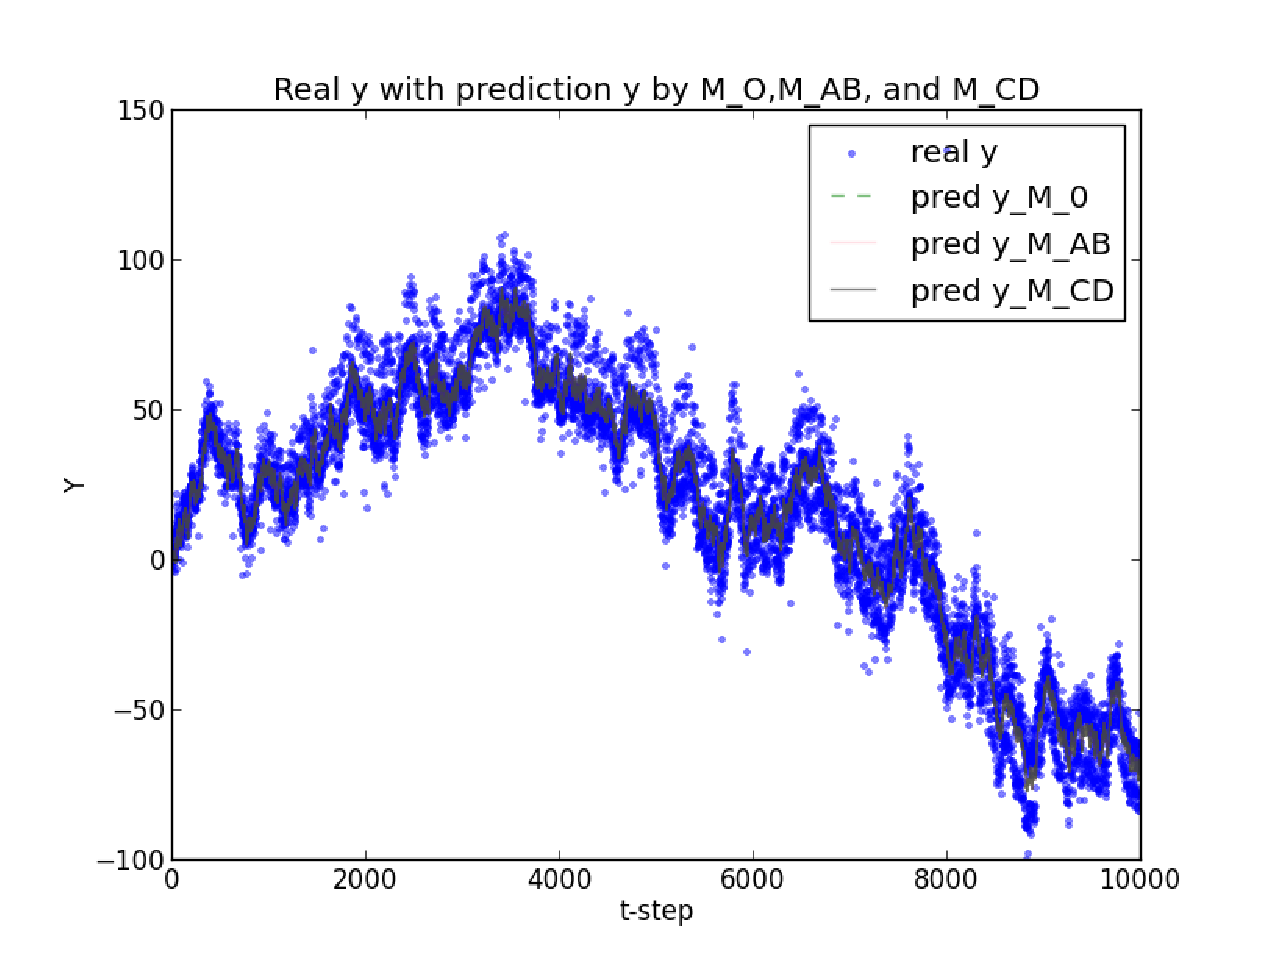
\includegraphics[width=12cm]{1a_graph.eps}
\caption{Real y with prediction y by $\Mc_0$,$\Mc_{AB}$,$\Mc_{CD}$}
\label{fig:aa}
\end{figure}
We also compute the loss function by using mean squared error $MSE$ of each model, where
$$
MSE=\sum^{10000}_{t=1}(y_{t,real}-X^{T}_{t}\mu_{t})^2
$$
we obtained the average of MSE by
$$
avgMSE=\frac{MSE}{10000}
$$
The result shows
$$
avgMSE(\Mc_0)=72.57644754, avgMSE(\Mc_{AB})=72.5764736, avgMSE(\Mc_{CD})=72.57657563
$$
We can find that
$$
avgMSE(\Mc_0)\approx avgMSE(\Mc_{AB}) \approx avgMSE(\Mc_{CD})
$$
Therefore, $\Mc_0,\Mc_{AB},\Mc_{CD}$ are approximately equivalent to each other.

\begin{framed}
\textbf{h. 15 points:} Recent issues with the company's communications infrastructure has caused some unusually noisy observations to be collected. Assuming that the error for observation $i$ is now defined by
\begin{equation}\label{}
\epsilon_i \sim \theta \Nc (0, \sigma^2) + (1-\theta) \Nc (0,50)
\end{equation}
Where $0<\theta<1$, what is the new posterior distribution over $\omega$ under this noise model at time $n$?
\end{framed}


Since $\epsilon_i$ is shown as formula (3), then by the property of linear combination of Gaussian distribution we have
$$
\epsilon_i \sim \Nc (\mu^{\ast}, (\sigma^{\ast})^2)
$$
in which
\begin{align*}
 & \mu^{\ast} = 0 \\
 & (\sigma^{\ast})^2 = \theta^2 \sigma^2 + (1- \theta)^2 50 \\
\end{align*}
Then the new posterior distribution over $\omega$ under this noise model at time $n$ is
$$
\Nc(Y_n | X_n^T \omega_n , (\sigma^{\ast})^2 + X_n^T \Sigma_n X_n)
$$

\clearpage








\end{document}
